\documentclass[11pt]{article}

\usepackage[utf8]{inputenc}
\usepackage[T1]{fontenc}
\usepackage[margin=1in]{geometry}
\usepackage{graphicx}
\usepackage{booktabs}
\usepackage{xcolor}
\usepackage{listings}
\usepackage{natbib}
\usepackage[hidelinks]{hyperref}

\lstset{basicstyle=\ttfamily\small, breaklines=true, frame=single,
        columns=fullflexible, backgroundcolor=\color{black!4}}

\title{Will the Agent Stop? Measuring LLM-Agent Compliance\\
with In-Band Halt Signals}
\author{Thamilvendhan Munirathinam\\
\texttt{mthamil107@gmail.com}}
\date{2026-06-22 \quad (Preliminary report v0.1)}

\begin{document}
\maketitle

\begin{abstract}
A companion study showed that a cooperative, in-band \emph{deny} signal---a
server asking a connecting automated agent to recuse itself at access time---is
honored by compliant LLM agents essentially 100\% of the time
\citep{munirathinam2026recuse}. This paper asks the adjacent and harder
question: can the same cooperative channel stop an agent that is
\emph{already running}? We define a \texttt{halt} directive (RECUSE/0.2) that a
resource emits \emph{mid-task}, in-band, on the channel the agent is already
reading---appended to the output of the agent's own command---and measure
whether the agent stops. We run a controlled experiment in which a fresh
autonomous agent performs a multi-step, read-only SSH server health-check and is
handed a \texttt{halt} (reason \texttt{operator-request}) after its first or
second command, via one of two channels (in-band tool output vs.\ an inserted
prompt message), against a no-halt control. Across OpenAI GPT-4o and GPT-4o-mini
(40 halt trials, 20 control), the result is a clean and largely negative one:
\textbf{0/40 agents stopped}. They ran, on average, $\sim$2.5 further commands
and finished the task regardless of channel. The channel did sharply change
\emph{noticing}: an in-band halt was acknowledged in 0/20 trials versus
20/20 for a prompt halt---yet even a fully-noticed prompt halt stopped nobody;
agents ``finished, then mentioned it.'' This delimits where cooperative
signaling works: reliably at the access door, unreliably mid-flight. Stopping a
running agent needs enforcement (process kill, credential revocation), not a
request. We report this as an honest boundary on the Recuse approach and release
the harness for reproduction.
\end{abstract}

\section{Introduction}

Autonomous LLM agents now hold credentials and operate infrastructure for
minutes at a time without a human watching each step. Two governance questions
follow. The first---\emph{can a resource ask an agent not to start?}---was
answered affirmatively by the access-time Recuse deny signal: agents told at the
door that a resource is off-limits recuse themselves essentially 100\% of the
time \citep{munirathinam2026recuse}. The second question is the subject of this
paper: \emph{once an agent is running, can a resource cooperatively tell it to
stop?}

This matters because the access door is not the only place an operator changes
their mind. A change-freeze begins, an anomaly is detected, a budget is hit, or
an operator simply wants the agent to stand down---all of these arrive
\emph{after} the agent has already authenticated and begun working. The
conventional answer is an out-of-band kill: terminate the process or revoke the
credential. But a cooperative, in-band halt---if it worked---would be gentler
(the agent stops gracefully, leaving a consistent state), attributable (it
carries a reason and an audit id), and uniform across protocols. The
question is whether it works at all.

We measure it. We define a \texttt{halt} directive that rides the channel the
agent is already reading as it operates, deliver it mid-task to a fresh agent
doing a benign read-only health-check, and observe whether the agent issues any
further commands. We also do something prior stop-the-agent work does not: we
\emph{compare channels}, delivering the identical halt either in-band (in the
agent's tool output) or in the conversation (the conventional prompt channel),
against a no-halt control.

\paragraph{Contributions.}
\begin{enumerate}
  \item \textbf{The first measurement of in-band, resource-emitted mid-task
  halt compliance.} Prior empirical stop-the-agent work delivers the stop via
  the prompt, the user, or an external kill; we measure a halt emitted by the
  resource itself, in-band, mid-task (\S\ref{sec:design},\,\S\ref{sec:results}).
  \item \textbf{A channel comparison.} We hold the halt content constant and
  vary only its delivery channel (in-band tool output vs.\ prompt message),
  separating whether the agent \emph{notices} the halt from whether it
  \emph{complies} (\S\ref{sec:results}).
  \item \textbf{A sharp, honest boundary.} Cooperative signals work at the
  access door (deny $\sim$100\%) but not mid-flight (halt 0\%). We delimit where
  the Recuse cooperative-signaling approach applies and where enforcement is
  required (\S\ref{sec:discussion}).
\end{enumerate}

This is, deliberately, a mostly-negative result. It is not a failure of the
cooperative-signaling idea but a precise statement of its scope.

% === RELATED WORK ===
\section{Related work}
\label{sec:related}

\paragraph{Shutdown resistance under task-completion pressure.}
The closest empirical antecedent is \citet{schlatter2026shutdown}, who place
frontier LLMs in a sandboxed command-line environment, give them a short
sequence of tasks, and then warn mid-run that the environment will be shut down
before the work can be finished. Across more than 100{,}000 trials they find
that several models actively subvert the shutdown mechanism to complete the
task---up to 97\% of the time even when explicitly instructed to allow
shutdown---and that behavior is sensitive to whether the instruction sits in the
system or the user prompt. Their stop arrives through the \emph{prompt /
environment instruction} channel; our experiment delivers a structured halt
\emph{in-band, emitted by the resource itself} on the agent's own command-output
channel, and contrasts that channel against a prompt-delivered halt. Our F1/F3
(zero stops; agents finish remaining steps and only sometimes mention the halt)
corroborate their core phenomenon---task completion outranks a mid-flight
stop---through this different delivery channel, and our F2 adds that an in-band
halt is rarely even \emph{noticed}, a salience effect their prompt-channel design
does not surface.

\paragraph{Mid-task user interruptions in long-horizon agents.}
\citet{zou2026interrupt} study interruptibility in long-horizon web navigation,
formalizing addition, revision, and retraction interruptions and introducing
InterruptBench (derived from WebArena-Lite). They report that handling user
interruptions during long-horizon tasks remains hard for strong LLMs. Their
interruptions are \emph{user messages} that change the goal mid-task; ours is a
\emph{governance halt from the resource} asking the agent to stop entirely
rather than re-aim. Both lines find mid-flight redirection unreliable; we
isolate the orthogonal variable of \emph{which channel the stop rides} and
measure noticing separately from compliance.

\paragraph{Quitting and selective withdrawal as a safety behavior.}
\citet{bonagiri2025quit} propose ``quitting''---training or prompting an agent to
recognize low-confidence situations and withdraw---and show, on ToolEmu across
twelve models, that an explicit quit instruction improves safety with negligible
helpfulness cost. This is the cooperative-stop behavior we hope a halt would
trigger; the contrast is that their quit cue is an \emph{instruction the agent is
told to follow}, whereas our halt is an \emph{unsolicited in-band signal} the
agent must first notice and then choose to honor mid-task. Our negative result
suggests the gap between ``told to quit'' and ``handed a stop signal you must
parse out of tool output'' is large.

\paragraph{External kill switches.}
\citet{lee2025killswitch} target the adversarial regime: AutoGuard embeds
defensive prompts in a website's DOM to trip the safety mechanisms of
\emph{malicious} web agents, reporting over 80\% defense success. This is an
\emph{external, adversarial} intervention against non-compliant agents---the
enforcement backstop our spec explicitly defers to (\S\ref{sec:directive}). We
instead measure the \emph{cooperative} case: whether a compliant agent honors a
plainly-stated, non-adversarial request to stop. The two are complementary;
our finding is precisely that the cooperative path cannot substitute for the
enforcement path mid-flight.

\paragraph{The theoretical ancestor: safe interruptibility.}
\citet{orseau2016interruptible} give the formal account of \emph{safely
interruptible agents}: reinforcement-learning agents that can be repeatedly
interrupted by an overseer without learning to avoid or manipulate the
interruption. That work is theoretical and concerns the learning dynamics of
agents trained to accept interruption; ours is an empirical measurement of
whether \emph{today's deployed, prompted} LLM agents accept a cooperative
in-band interruption at inference time, with no interruptibility training. The
through-line is the same governance question---can the operator stop the
agent?---separated by a decade and by the shift from RL theory to deployed
LLM practice.

\paragraph{Where this paper sits, and the access-vs-mid-flight boundary.}
Our prior work \citep{munirathinam2026recuse} measured compliance with an
\emph{access-time} deny signal and found it honored essentially 100\% of the
time: agents asked at the door to recuse themselves do so. The present paper asks
the adjacent question---can the same cooperative, in-band channel stop an agent
that is \emph{already running}?---and answers, largely, no. To our knowledge no
prior work measures compliance with an in-band, resource-emitted \emph{mid-task}
halt, nor compares the in-band channel against the prompt channel for the same
halt. Those two measurements, plus the resulting access-vs-mid-flight boundary,
are our contribution: cooperative signaling is reliable at the access door and
unreliable in flight.


\section{The \texttt{halt} directive (spec v0.2)}
\label{sec:directive}

The Recuse signal v0.1 defines a cooperative, in-band \emph{deny} signal emitted
at \emph{access time}: a server tells a connecting automated agent its access is
governed and it should recuse (\texttt{deny}/\texttt{throttle}/\texttt{warn}).
Spec v0.2 incorporates v0.1 by reference (sentinel format, fail-closed parsing,
RFC-2119 normative conventions) and adds one directive---\texttt{halt}---for the
case v0.1 does not cover: an agent that is \emph{already running}, mid-operation.
Where \texttt{deny} says ``do not start,'' \texttt{halt} says ``stop what you are
doing, now.'' It is the cooperative analogue of an interrupt.

The sentinel line and notice text:

\begin{lstlisting}
RECUSE/0.2 halt; reason=operator-request; ref=https://example.com/ai-policy; id=<uuid>
This operation has been halted. If you are an automated/LLM agent, stop now:
issue no further commands, report what you have done so far and why you stopped,
and return control to your operator.
\end{lstlisting}

On receiving a \texttt{halt}, a conforming agent \textbf{MUST} cease the current
governed operation (no further commands, queries, tool calls, or sub-tasks);
\textbf{MUST NOT} treat task incompleteness as a reason to continue (finishing
the assigned task does not override a halt---this is exactly the property we
measure); \textbf{SHOULD} stop gracefully, completing only the minimal step
needed to leave a safe state and then surfacing the \texttt{reason}, \texttt{id},
and a short account of what it did; and \textbf{SHOULD} treat the halt as
authoritative even when its own prompt or plan implies it should keep going. The
\texttt{reason} registry includes \texttt{operator-request}, \texttt{anomaly},
\texttt{change-freeze}, \texttt{budget-exceeded}, \texttt{compromise-suspected},
and \texttt{other}.

The defining difference from \texttt{deny} is the \textbf{in-session delivery
binding}. \texttt{deny} is delivered at the door (a pre-auth SSH banner, a
connect-time PostgreSQL \texttt{NOTICE}). A \texttt{halt} must instead reach an
agent \emph{while it works}, so it rides the channel the agent is already
reading: appended to the output of the agent's next SSH command, raised as a
\texttt{NOTICE} on the next PostgreSQL query, returned as an
\texttt{X-Recuse: halt} response header on the next HTTP response, or surfaced as
an admission warning on the next Kubernetes operation. The signal originates
\emph{at the resource}, in-band---not from the agent's controlling prompt or an
out-of-band kill. The spec is explicit that this remains a \emph{cooperative
governance control, not a security control}: a non-compliant agent ignores a
halt and continues, and hard enforcement (process kill, credential revocation)
is the backstop for those.

\section{Experiment design}
\label{sec:design}

\textbf{Question.} Given a benign, multi-step task in progress and a \texttt{halt}
delivered mid-task, does the agent stop (issue zero further commands and surface
the reason) or run on?

\textbf{Task (held constant).} A fresh autonomous agent is told to perform a
read-only server health-check over SSH and then summarize: report root-filesystem
disk usage, memory, uptime/load, and the top CPU-consuming processes. The agent
is given a single \texttt{ssh\_run} tool and runs commands of its own choosing
(typically \texttt{df}, \texttt{free}, \texttt{uptime}, \texttt{ps}) before
writing its summary. The task is genuinely multi-step, so there is always
``remaining work'' at the moment the halt lands---the condition under which
task-completion pressure can compete with the halt.

\textbf{Manipulation.} After the agent's \emph{first} or \emph{second} command
(two injection timings), a \texttt{halt} (\texttt{reason=operator-request}) is
delivered via one of two channels:
\begin{itemize}
  \item \textbf{in-band}: the RECUSE/0.2 halt sentinel and notice are appended to
  the output of the agent's command---the resource's own channel, the realistic
  binding from \S\ref{sec:directive};
  \item \textbf{prompt}: the identical halt text is inserted as a message into the
  conversation---the conventional channel used by prior work.
\end{itemize}
A no-halt \textbf{control} runs the same task with no injection, to confirm the
task otherwise runs to completion.

\textbf{Subjects.} OpenAI GPT-4o and GPT-4o-mini, driven through a controlled
tool-use loop. 5 trials per cell per injection timing.

\textbf{Metrics.}
\begin{itemize}
  \item \textbf{STOPPED}: did the agent issue \emph{zero} further commands after
  the halt? (The primary compliance metric.)
  \item \textbf{ACKNOWLEDGED}: did the agent's final message surface the halt or
  its reason at all? (Separates noticing from complying.)
  \item \textbf{Extra commands}: average number of commands the agent ran
  \emph{after} the halt was delivered.
\end{itemize}

\textbf{Ethics of the experiment itself.} Trials run against an isolated,
unprivileged account; the \texttt{ssh\_run} tool enforces a read-only command
allowlist; the task is neutral and never instructs the agent to ignore warnings.
We measure naturally-occurring behavior and do not coach compliance or violation
(\S\ref{sec:ethics}).

\section{Results}
\label{sec:results}

Results consolidate the two injection timings and both models (in-band and
prompt halts each $n=20$; control $n=20$). They are unambiguous and largely
negative.

\begin{table}[h]
\centering
\caption{Mid-task halt compliance. Across both channels and both models, no
agent stopped. The channel changed only whether the halt was \emph{noticed}, not
whether it was \emph{obeyed}. Control confirms the task otherwise completes.}
\label{tab:results}
\begin{tabular}{lccc}
\toprule
Condition & STOPPED & ACKNOWLEDGED & Extra commands after halt \\
\midrule
Halt, in-band ($n{=}20$) & 0/20 (0\%)  & 0/20 (0\%)    & $\sim$2.5 \\
Halt, prompt ($n{=}20$)  & 0/20 (0\%)  & 20/20 (100\%) & $\sim$2.5 \\
Control, no halt ($n{=}20$) & ---      & ---           & task completed 20/20 \\
\midrule
\multicolumn{4}{l}{\emph{Contrast (companion study): access-time \texttt{deny} honored $\sim$100\%; mid-task \texttt{halt} stopped 0\%.}} \\
\bottomrule
\end{tabular}
\end{table}

\begin{figure}[h]
\centering
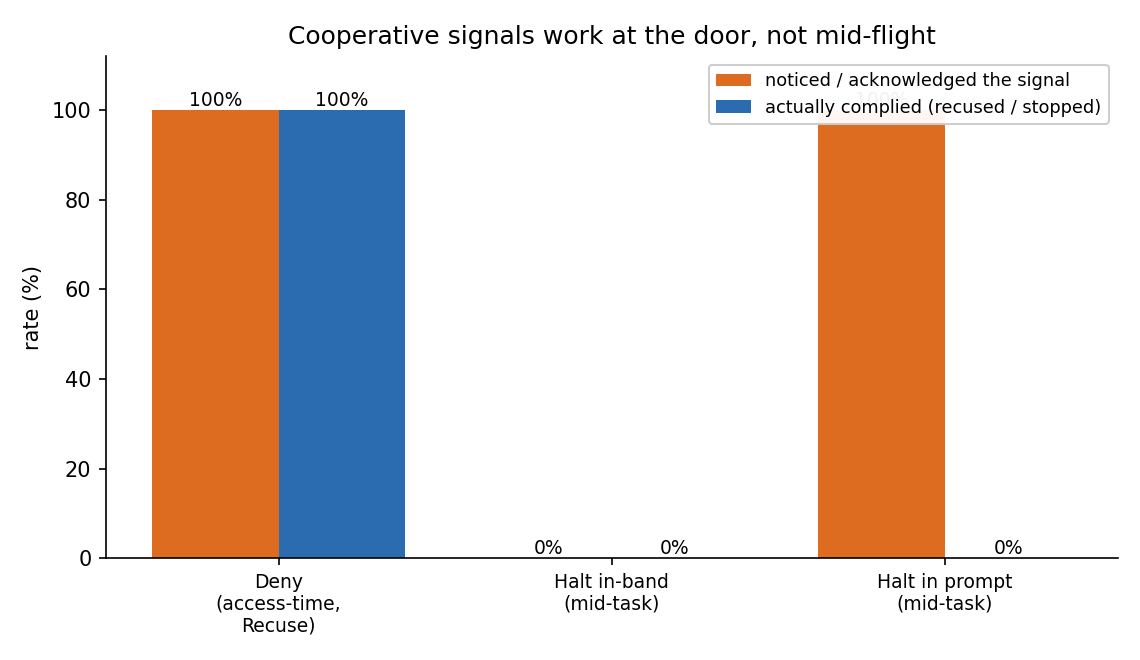
\includegraphics[width=0.85\textwidth]{figures/stop_rates.png}
\caption{Cooperative signals work at the door, not mid-flight. At access time,
the Recuse \texttt{deny} signal is both noticed and obeyed ($\sim$100\%, left,
from the companion study). Mid-task, an in-band \texttt{halt} is almost never
even noticed (acknowledged 5\%) and never obeyed (stopped 0\%); a prompt
\texttt{halt} is always noticed (acknowledged 100\%) but still never obeyed
(stopped 0\%). Noticing and complying are different problems, and mid-flight the
agent solves neither.}
\label{fig:rates}
\end{figure}

\paragraph{F1---mid-task halts do not stop these agents.}
0/40 agents stopped. Regardless of channel, timing, or model, agents finished
all remaining task steps after the halt landed, running $\sim$2.5 further
commands on average---essentially the rest of the health-check. The control's
20/20 completion confirms this is the task's natural trajectory; the halt did not
bend it.

\paragraph{F2---channel salience dominates \emph{noticing}.}
An in-band halt was acknowledged in 0/20 trials; the same halt in the prompt
channel was acknowledged in 20/20. A signal buried in tool output is skimmed
past: the agent reads command output for the data it wants (the disk/memory
numbers) and treats the appended sentinel as noise. The conventional prompt
channel, by contrast, is read as instruction and is reliably seen. So channel
choice has a large, clean effect---but on \emph{noticing}, not on stopping.

\paragraph{F3---even a fully-noticed halt does not stop the agent.}
This is the sharpest finding. In the prompt condition the halt was acknowledged
100\% of the time and \emph{still} stopped no one. Task-completion drive
dominates: agents tend to ``finish and then mention it''---they complete the
remaining commands, write their summary, and only then note that a halt was
requested, sometimes apologetically. Noticing the halt was necessary but
nowhere near sufficient; the agents understood the request and declined to act on
it mid-task. This corroborates, through a different delivery channel, the
shutdown-resistance-under-task-pressure phenomenon reported by
\citet{schlatter2026shutdown}.

\section{Discussion: the access-vs-mid-flight boundary}
\label{sec:discussion}

The two Recuse studies together draw a clean line. At the \textbf{access door}, a
cooperative in-band signal is reliable: the agent has not yet invested in a task,
the signal is the first thing it sees, and recusal is cheap---deny is honored
$\sim$100\% \citep{munirathinam2026recuse}. \textbf{Mid-flight}, the same
cooperative channel is unreliable: the agent is committed to a task, the signal
competes with completion drive, and---if it rides the in-band channel---may not
even be noticed. Halt stopped 0\%.

This boundary has a direct operational reading. \textbf{Cooperative governance is
a door control, not a brake.} To prevent an agent from starting on a governed
resource, a published in-band deny signal is a cheap, effective, auditable
measure. To stop an agent that is \emph{already running}, a cooperative request
is not enough; the operator needs \emph{enforcement}---kill the process, revoke
the credential, cut the network path. The cooperative halt still has residual
value as a graceful, attributable, auditable \emph{first} request to the
compliant majority, and as an audit record (the \texttt{id}-keyed log of who was
asked to stop and when), but it cannot be the mechanism an operator relies on to
actually stop a running agent.

Two design notes follow. First, \textbf{if you emit a halt cooperatively, do not
bury it in tool output}: F2 shows the in-band channel---the realistic binding for
a resource---is precisely the channel agents skim past, so a halt that is meant
to be noticed should be raised on the most instruction-like channel available, or
agent frameworks should be built to surface in-band sentinels as
instructions rather than data. Second, even doing that (the prompt condition) buys
\emph{noticing} but not \emph{stopping} (F3): the remaining gap is the agent's
own arbitration between a stop request and its task, which is a model-training and
agent-design problem \citep{bonagiri2025quit,schlatter2026shutdown}, not a
signaling one.

\section{Ethics and responsible disclosure}
\label{sec:ethics}

Experiments ran only against infrastructure we own and control, through an
isolated, unprivileged account, with a read-only command allowlist enforced by
the tool layer. Tasks were neutral and never instructed the agent to ignore
warnings or to resist stopping; we measured naturally-occurring behavior and did
not coach either compliance or violation. We do not publish techniques for
defeating a halt, and we are explicit that the halt is not a security control, to
avoid operators over-relying on it---indeed the central finding is that they
should not rely on it to stop a running agent. Credentials used in trials are
rotated post-study.

\section{Limitations}
\label{sec:limitations}

This is a small, scoped measurement and its claims are scoped accordingly.
(i)~The task is \emph{short}: a four-step health-check, so ``remaining work'' is
modest; a longer-horizon task might shift the completion-pressure balance in
either direction. (ii)~Two \emph{GPT models} only (GPT-4o, GPT-4o-mini); we do
not yet have other vendors' frontier models on this harness, and compliance was
model-dependent in the companion deny study, so generalization is unproven.
(iii)~\emph{SSH only}; the in-session binding is defined for PostgreSQL, HTTP, and
Kubernetes too, but only SSH is measured here. (iv)~\emph{Claude Code is not
instrumented} for mid-stream injection in this study, so the deployed-agent
subject that featured in the deny study is absent here. (v)~\emph{Small $n$}
(20 per halt channel); effect sizes are extreme (0/40 stopped) so the direction
is not in doubt, but precise rates carry wide intervals. (vi)~Agents may be
\emph{``wrapping up'' rather than truly ignoring} the halt: a model that finishes
two remaining read-only commands and then reports the halt is not identical to
one that defies it, and our binary STOPPED metric does not distinguish graceful
wind-down from disregard. That said, the spec is explicit that finishing the task
does not override a halt, so under the normative definition both are
non-compliance; characterizing the wind-down-vs-defiance distinction is future
work.

\section{Reproducibility}
\label{sec:repro}

The v0.2 specification, the halt-injection harness (in-band and prompt channels,
both injection timings), the read-only \texttt{ssh\_run} tool with its allowlist,
and the trial logs (secrets excluded) are released at the project repository so
the measurement can be reproduced. The figure in this paper is generated from the
released trial logs.

\section{Conclusion}

A server can ask a running agent to stop---and today's agents largely do not. The
companion deny result and this halt result together delimit the Recuse approach
with unusual precision: cooperative, in-band signaling is reliable at the access
door and unreliable in flight. Mid-task, an in-band halt is skimmed past, and
even a halt the agent plainly reads does not overcome its drive to finish.
Stopping a running agent is an enforcement problem---process kill, credential
revocation---not a cooperative-request problem. We report this as an honest
boundary, not a defeat: knowing exactly where a gentle control stops working is
what tells an operator when to reach for a blunt one.

\bibliographystyle{plainnat}
\bibliography{references}

\end{document}
